\documentclass[a4paper, 11pt, twoside]{article}

%\usepackage[ngerman]{babel}
\usepackage[english]{babel}
\usepackage[latin1]{inputenc}

\usepackage{graphicx,float}
%\usepackage{pifont}
\usepackage{type1cm}
\usepackage{amssymb, amsthm, amsmath}
\usepackage{listings}
\usepackage{pgf}
\usepackage{tikz}
\usetikzlibrary{shapes.geometric}
\usepackage{url}
\usepackage{hyperref}

\usepackage{makeidx}
\makeindex

\setlength{\parindent}{0em}
\setlength{\oddsidemargin}{0.0cm}
\setlength{\evensidemargin}{0.0cm}
\setlength{\textheight}{24.0cm}
\setlength{\topmargin}{-1.0cm}
\setlength{\footskip}{1.5cm}
\setlength{\textwidth}{15.5cm}

\renewcommand*\familydefault{\sfdefault}
\newcommand{\dd}{\mathrm{d}}
\newtheorem{problem}{Problem}[section]
\newtheorem{theorem}{Theorem}[section]
\newtheorem{remark}{Remark}[section]

\bibliographystyle{unsrt}

\begin{document}
\pagestyle{empty}
%\documentclass[a4paper]{article}

%\usepackage{pgf}
%\usepackage{graphicx}
%\usepackage{pifont}
%\usepackage{type1cm}

\setlength{\textwidth}{14cm}
\setlength{\oddsidemargin}{1cm}

%\begin{document}

\pagestyle{empty}

%%%%%%%%%%%%%%%%%%%%%%%%%%%%%%%%%%%%%%%%
%%%%%%%%%%%%%%%%%%%%%%%%%%%%%%%%%%%%%%%%
%%%%%%%%%%%%%%%%%%%%%%%%%%%%%%%%%%%%%%%%

\newcount \Z
\Z=20

%%% logos %%%

%%% NUMHPC %%%
\newlength{\numhpclogox}
\setlength{\numhpclogox}{\paperwidth} % 20/210ths of the paperwidth
\divide\numhpclogox by 210
\multiply\numhpclogox by 100

\newlength{\numhpclogoy}
\setlength{\numhpclogoy}{\paperheight} % 270/297ths of the paperwidth
\divide \numhpclogoy by 297
\multiply \numhpclogoy by -235

\newlength{\numhpclogoheight}
\setlength{\numhpclogoheight}{\paperheight} % 270/297ths of the paperwidth
\divide\numhpclogoheight by 297
\multiply\numhpclogoheight by 20

%%% KIT %%%
\newlength{\kitlogox}
\setlength{\kitlogox}{\paperwidth} % 20/210ths of the paperwidth
\divide\kitlogox by 210
\multiply\kitlogox by 0

\newlength{\kitlogoy}
\setlength{\kitlogoy}{\paperheight} % 270/297ths of the paperwidth
\divide \kitlogoy by 297
\multiply \kitlogoy by -230

\newlength{\kitlogoheight}
\setlength{\kitlogoheight}{\paperheight} % 270/297ths of the paperwidth
\divide\kitlogoheight by 297
\multiply\kitlogoheight by 15


%%% EMCL %%%
\newlength{\emcllogox}
\setlength{\emcllogox}{\paperwidth} % 20/210ths of the paperwidth
\divide\emcllogox by 210
\multiply\emcllogox by 28

\newlength{\emcllogoy}
\setlength{\emcllogoy}{\paperheight} % 270/297ths of the paperwidth
\divide \emcllogoy by 297
\multiply \emcllogoy by -160

\newlength{\emcllogoheight}
\setlength{\emcllogoheight}{\paperheight} % 270/297ths of the paperwidth
\divide\emcllogoheight by 297
\multiply\emcllogoheight by 20

%%% HIFLOW %%%
\newlength{\hiflowlogox}
\setlength{\hiflowlogox}{\paperwidth} % 20/210ths of the paperwidth
\divide\hiflowlogox by 210
\multiply\hiflowlogox by 28

\newlength{\hiflowlogoy}
\setlength{\hiflowlogoy}{\paperheight} % 270/297ths of the paperwidth
\divide \hiflowlogoy by 297
\multiply \hiflowlogoy by -160

\newlength{\hiflowlogoheight}
\setlength{\hiflowlogoheight}{\paperheight} % 270/297ths of the paperwidth
\divide\hiflowlogoheight by 297
\multiply\hiflowlogoheight by 33

%%%%%%%%%%%%%%%%%%%%%%%%%%%%%%%%%%%%%%%%
%%%%%%%%%%%%%%%%%%%%%%%%%%%%%%%%%%%%%%%%
%%%%%%%%%%%%%%%%%%%%%%%%%%%%%%%%%%%%%%%%

%%% NUMHPC %%%
%%\pgftext[bottom, left, at={\pgfpointadd{\pgfpoint{0pt}{0pt}}{\pgfpoint{\numhpclogox}{\numhpclogoy}}}]{\includegraphics[totalheight=\numhpclogoheight]{numhpc}}

%%% KIT %%%
%%\pgftext[bottom, left, at={\pgfpointadd{\pgfpoint{0pt}{0pt}}{\pgfpoint{\kitlogox}{\kitlogoy}}}]{\includegraphics[totalheight=\kitlogoheight]{kitlogo}}

%%% EMCL %%%
\pgftext[bottom, left, at={\pgfpointadd{\pgfpoint{0pt}{0pt}}{\pgfpoint{\hiflowlogox}{\hiflowlogoy}}}]{
\includegraphics[totalheight=\hiflowlogoheight]{HF3_color}}

%%% horizontal lines %%%
\pgfline{\pgfxy(-1pt,0.1pt)}{\pgfxy(15pt,0.1pt)}
\pgfline{\pgfxy(-1pt,-21.4pt)}{\pgfxy(15pt,-21.4pt)}
%%\pgfline{\pgfxy(-1pt,-22.4pt)}{\pgfxy(15pt,-22.4pt)}

%%% EMCL text %%%
\pgftext[bottom, left, at={\pgfpointadd{\pgfpoint{0pt}{0pt}}{\pgfpoint{0cm}{1cm}}}]{{\LARGE{{\bf Tutorial}}}}

%%% EMCL web %%%
\pgftext[bottom, left, at={\pgfpointadd{\pgfpoint{0pt}{0pt}}{\pgfpoint{10.5cm}{-21.7cm}}}]{{\fontsize{13}{10}\selectfont{} http://www.hiflow3.org/}}

\hspace{2cm}
\begin{picture}(0,0)(-250,-25)

\includegraphics[scale=.22]{emcl.pdf} 
\end{picture}

%%% author %%%
\pgftext[bottom, left, at={\pgfpointadd{\pgfpoint{0pt}{0pt}}{\pgfpoint{0cm}{-4cm}}}]{{
\begin{parbox}{13cm}{
\begin{center}\fontsize{12}{30}\selectfont{} J. Roller, C. Song
\end{center}}
\end{parbox}}}

%%% title %%%
\pgftext[bottom, left, at={\pgfpointadd{\pgfpoint{0pt}{0pt}}{\pgfpoint{0cm}{-7.5cm}}}]{{
\begin{parbox}{13cm}{
%%\begin{center}\fontsize{18}{30}\selectfont{} \bf Using HiFlow$^3$ for solving the
\begin{center}\fontsize{22}{30}\selectfont{} \bf Large Eddy Simulation
\end{center}}
\end{parbox}}}

%%% date %%%
\pgftext[bottom, left, at={\pgfpointadd{\pgfpoint{0pt}{0pt}}{\pgfpoint{0cm}{-16.4cm}}}]{{
\begin{parbox}{13cm}{
\begin{center}\fontsize{12}{24}\selectfont{} 
\vspace{5cm}
\textit{modified on \today}\\ 
\vspace{6.5cm}
\hspace{6cm}\textit{Version 1.3}
\end{center}}
\end{parbox}}}

%fhfh \hfill sjdh

%\end{document}


%\newpage
%\null\newpage

\tableofcontents

\newpage
\pagestyle{plain}
\framebox[15.5cm]{\parbox[c][2.3cm]{14.5cm}{
{\fontsize{19}{19}\selectfont{} \bf{Using HiFlow$^3$ for simulating\\[0.5em] turbulent incompressible flows}
}}}
\vspace{0.5cm}
\section{Introduction}

HiFlow$^3$ is a multi-purpose finite element software providing powerful tools for efficient and accurate solution of a wide range of problems modeled by partial differential equations (PDEs). Based on object-oriented concepts and the full capabilities of C++ the HiFlow$^3$ project follows a modular and generic approach for building efficient parallel numerical solvers. It provides highly capable modules dealing with the mesh setup, finite element spaces, degrees of freedom, linear algebra routines, numerical solvers, and output data for visualization. Parallelism - as the basis for high performance simulations on modern computing systems - is introduced on two levels: coarse-grained parallelism by means of distributed grids and distributed data structures, and fine-grained parallelism by means of platform-optimized linear algebra back-ends.

\subsection{How to Use the Tutorial?}
You find the example code (les\_tutorial.cc, les\_tutorial.h) and a parameter file for the first numerical example (les\_tutorial.xml) in the folder \verb'/hiflow/examples/les'. The geometry data (*.inp, *.vtu) is stored in the folder \verb'/hiflow/examples/data'.

\subsubsection{Using HiFlow$^3$ as a Developer}\label{sectiondeveloper}
First build and compile HiFlow$^3$. Go to the directory \verb'/build/examples/les', where the binary \textbf{les\_tutorial} is stored. Type \textbf{./les\_tutorial}, to execute the program in sequential mode. To execute in parallel mode \index{program!executing in parallel} with four processes, type \textbf{mpirun -np 4 ./les\_tutorial}. In both cases, you need to make sure that the default parameterfile les\_tutorial.xml is stored in the same directory as the binary, and that the geometry data specified in the parameter file is stored in \verb'/hiflow/examples/data'. Alternatively, you can specify the path of your own xml-file with the name of your xml-file (first) and the path of your geometry data (second) in the comment line, i.e. \textbf{./les\_tutorial} \verb'/"path_to_parameterfile"/"name_of_parameterfile".xml' \verb'/"path_to_geometry_data"/'.

\section{Mathematical Setup}

\subsection{Problem}

We consider the simulation of an instationary flow in a two-dimensional cavity with the moving lid $\Gamma_{\text{in}}$. 
\setlength{\unitlength}{1cm}
\begin{figure}[!h]
	\centering
		\begin{tikzpicture}[square/.style={regular polygon,regular polygon sides=4}]
        \draw (0,0) -- node[left] {$\Gamma_{0}$} (0,5);
        \draw (0,5) --  node[above] {$\Gamma_{\text{in}}$} (5,5);
        \draw (5,5) -- node[right] {$\Gamma_{0}$}(5,0);
        \draw (5,0) -- node[below] {$\Gamma_{0}$} (0,0);
        \draw[->](0,-0.8) -- node[below] {$1.0$} (5.0,-0.8);
        \draw[->](5.0,-0.8) -- (0.0,-0.8);
        \draw[->](-0.8,0) -- (-0.8,5.0);
        \draw[->](-0.8,5.0) -- node[left] {$1.0$} (-0.8,0.0);
    \end{tikzpicture}
\caption{Unit square with moving lid $\Gamma_{\text{in}}$.}
\label{channel}
\end{figure}
We assume the liquid to be an incompressible Newtonian fluid, and model the flow by the Navier-Stokes equations.\index{equation!Navier-Stokes} We have to distinguish two different boundary conditions, namely, (\ref{NR1}) the inflow condition at  $\Gamma_{\text{in}}$ and 
(\ref{NR2}) the no-slip condition
at all remaining parts of the boundary $\Gamma_0$. We consider the following initial-boundary value problem for the unknown velocity field $u = (u_1(x_1, x_2), u_2(x_1,x_2))^T$ and the unknown pressure $p = p(x_1, x_2)$ of the velocity field:


\begin{subequations}
\begin{align}
\label{eq:NS_strong1}
\partial_t u  + (u \cdot \nabla ) u -\nu \Delta u + \frac{1}{\rho} \nabla p &= 0, \quad \text{ in } \Omega,\\
\label{eq:NS_strong2}
\nabla \cdot u &= 0, \quad \text{ in } \Omega,\\
\label{NR1}
u &= g, \quad \text{ on } \Gamma_{\text{in}},\\ 
\label{NR2}
u &= 0, \quad \text{ on } \partial\Omega \backslash \overline{\Gamma_{\text{in}}}=:\Gamma_0, \\
\label{eq:NR3}
u(0,\cdot) &= u_0, \hspace{0.35cm} \mathrm{in } \hspace{0.1cm} \Omega
\end{align} 
\end{subequations}  

where $\Omega$ is the domain specified in Fig \ref{channel}. The viscosity\index{viscosity} $\nu = \nu(x_1, x_2)$ is a known material constant and the density\index{density} $\rho = \rho(x_1, x_2)$ is also constant due to the incompressibility of the fluid, $g:\Gamma_{\text{in}}\rightarrow \mathbb{R}$ is a given Dirichlet data. 

\subsection{Turbulence models}
 For the case of high Reynolds numbers \index{Reynolds number}, we have to take into account the occurrence of turbulent phenomena (eddies). The complexity of these can be characterized by their dependence on many different spatial scales. A finite element simulation of the Navier-Stokes equations can only simulate eddies up to the associated mesh size, which implies that an extremely fine mesh size is generally needed to directly simulate turbulent flows. However, on a fixed-size mesh, we can construct a splitting of the solution
 
 \begin{equation}
    u = \bar{u} + u', \hspace{0.5cm} p = \bar{p} + p',
\end{equation} 

such that $(\bar{u},\bar{p})$ are regarded as the \textit{large} or \textit{resolved} scale parts and $(u',p')$ are the \textit{small} or \textit{subgrid-scale} (SGS) \index{subgrid-scale (SGS)} parts of $(u,p)$. The large eddy simulation (LES) \index{large eddy simulation (LES)} approach then consists of applying a convolution with a \textit{spatial filter} $g$ \index{filter!spatial} to the Navier-Stokes equations with the aim of "filtering out" the small scales (which are then \textit{modeled}, not simulated) and simulating the filtered equations \index{equation!filtered}. These are given by

\begin{subequations}
\begin{align}
\label{eq:SANS_strong1}
\partial_t \bar{u} + \nabla \cdot (\overline{uu^T}) - \nu \Delta \bar{u} + \nabla \frac{1}{\rho}\bar{p} &= \bar{f} \hspace{0.3cm} \mathrm{in } \hspace{0.1cm} (0,T] \times \mathbb{R}^d, \tag{3a} \\ \label{eq:SANS_strong2}
\nabla \cdot \bar{u} &= 0 \hspace{0.35cm} \mathrm{in } \hspace{0.1cm} (0,T] \times \mathbb{R}^d, \tag{3b} \\
\bar{u}(0,\cdot) &= \bar{u}_0 \hspace{0.15cm}\mathrm{in } \hspace{0.1cm} \mathbb{R}^d. \tag{3c} \label{eq:SANS_strong3}
\end{align}
\end{subequations}
    

The advective term \index{advective term} $\nabla \cdot (\overline{uu^T})$ in (\ref{eq:SANS_strong1}) gives rise to the LES \textit{closure problem} \index{closure problem} because we need to find a model that expresses it in terms of $\bar{u}$. Assuming linearity of the filter, it can be written as \begin{equation}
\label{eq:adv}
    \overline{uu^T} = \overline{\bar{u}\bar{u}^T} + \overline{\bar{u}u'^T} + \overline{u'\bar{u}^T} + \overline{u'u'^T}.
\end{equation}
On the right-hand size the second and third term are the large-scale and \textit{cross terms}, and the last term corresponding to SGS advection. The approach followed here assumes a Gaussian filter \index{filter!Gaussian} and consists of Fourier transforming each term, applying a rational approximation \index{rational!approximation} and then inverting the Fourier transform \cite[p.541-551]{John}. With a second-order approximation, we get for the large-scale and cross terms \begin{equation}
\label{eq:rat1}
    \overline{\bar{u}\bar{u}^T} + \overline{\bar{u}u'^T} + \overline{u'\bar{u}^T} \approx \bar{u}\bar{u}^T + \big(I - \frac{\delta^2}{24}\Delta\big)^{-1}\frac{\delta^2}{12}\nabla \bar{u} \nabla \bar{u}^T,
\end{equation} where $\delta$ is the \textit{characteristic filter width} \index{characteristic filter width} which should refer to all eddies of size $\mathcal{O}(\delta)$ being filtered out. Commonly $\delta := 2h$ with the local mesh size $h$. We set \begin{equation}
    h := h_{K,\text{min}},
\end{equation} where $h_{K,\text{min}}$ is the shortest edge on an individual mesh cell $K$. The second term on the right-hand side of (\ref{eq:rat1}) defines a tensor-valued elliptic auxiliary problem \index{auxiliary problem} \begin{equation}
\label{eq:rat2}
    -\frac{\delta^2}{24}\Delta \mathbb{X} + \mathbb{X} = \frac{\delta^2}{12}\nabla \bar{u} \nabla \bar{u}^T
\end{equation} which we equip with homogeneous Neumann boundary conditions. Equations (\ref{eq:rat1}),(\ref{eq:rat2}) then give the (second order) \textbf{rational LES model} \index{rational!LES model}. As the term $(I-\frac{\delta^2}{24}\Delta)^{-1}$ approximates convolution with a Gaussian filter, the model can alternatively be defined by \begin{equation}
\label{eq:ratconv}
    \overline{\bar{u}\bar{u}^T} + \overline{\bar{u}u'^T} + \overline{u'\bar{u}^T} \approx \bar{u}\bar{u}^T + \frac{\delta^2}{12}g*(\nabla \bar{u} \nabla \bar{u}^T).
\end{equation} A major drawback of this model is that it approximates the SGS term $\overline{\bar{u}'\bar{u}'^T}$ as zero. Because completely neglecting this term is physically unreasonable, we need to add an SGS model which we call the \textit{turbulent} or \textit{eddy viscosity} \index{viscosity!turbulent} \index{viscosity!eddy} $\nu_T(\bar{u})$. The most popular choice is the \textbf{Smagorinsky model} \cite{Smagorinsky} 

\begin{equation}
\label{eq:Smagorinsky}
    \nu_T(\bar{u}) = C_S \delta^2 ||\nabla\bar{u}||_F
\end{equation} 

with the \textit{Smagorinsky constant} \index{Smagorinsky!constant} $C_S$ which is not generally known. It has been estimated to be roughly $0.17$ for isotropic turbulence. Another model derived by Iliescu and Layton (\textbf{IL}) in \cite{Iliescu} is given by 

\begin{equation}
\label{eq:IL}
    \nu_T(\bar{u}) = C_S \delta ||\bar{u} - g * \bar u||_2.
\end{equation} 

This model can also be defined with a rational approximation of the convolution with the Gaussian filter, yielding 

\begin{equation}
    \nu_T(\bar{u}) = C_S \delta ||\bar{u} - (I-\frac{\delta^2}{24}\Delta)^{-1} \bar u||_2 \label{eq:iliLayton}
\end{equation} 

and another auxiliary problem \index{auxiliary problem} with right-hand side $\bar{u}$. It is one of three models proposed in \cite{Iliescu}, two of which have been implemented in this tutorial. In numerical experiments, the scaling factor $C_S$ seems to need a larger value than for the Smagorinsky model. The likely reason is that the Smagorinsky model, unlike the Iliescu-Layton model, is often defined with a squared constant instead. Thus, it roughly holds that \begin{equation}
    C_{S, \text{IL}} \approx \sqrt{C_{S, \text{Smag.}}}.
\end{equation} Because we replace $\bar{u}$ with the previous time step velocity $\bar{u}_k$ in the auxiliary problems, these only have to be solved once in each time step. In the paper \cite{Akin}, the \textbf{streamline-upwind Petrov-Galerkin (SUPG)} \index{streamline-upwind Petrov-Galerkin (SUPG)} method was compared to the Smagorinsky model. We can define a corresponding eddy viscosity \index{viscosity!eddy} by 

\begin{equation}
\label{eq:SUPG}
    \nu_{T,K}(\bar{u}) = \tau_{\mathrm{SUPG}} ||\bar{u}||_{\infty,K}^2
\end{equation} 
with the SUPG stabilization parameter $\tau_{\mathrm{SUPG}}$ and the point-wise maximum of $u$ in the Euclidean norm 

\begin{equation}
    ||\bar{u}||_{\infty,K} = \max\big\{\sqrt{\bar{u} \cdot \bar{u}}, \hspace{0.1cm} x \in K\big\}
\end{equation} 

for any mesh cell $K$. This model, unlike all previous models, is based on the weak formulation, as it arises from the SUPG method. Vreman \cite{Vreman} introduced a sophisticated eddy viscosity model in 2004. It vanishes identically for over 300 types of non-turbulent flow structures, a considerable improvement over the Smagorinsky model, which is overly diffusive for laminar flows. In three spatial dimensions, Vreman's eddy viscosity is given by \begin{equation}
    \label{eq:Vreman}
    \nu_T := \begin{cases}
    C_S \delta^2 \sqrt{\frac{B}{|\nabla \bar{u}|_F^4}}, & |\nabla \bar{u}|_F^4 > 0 \\
    0, & \text{else}.
    \end{cases}
\end{equation} Using the shorthand $\beta$ for the velocity gradient times its transpose \begin{equation}
    \beta_{i,j} := (\nabla \bar{u} \nabla \bar{u}^T)_{i,j}, 
\end{equation} the scalar function $B(\beta)$ is defined as \begin{equation}
    B(\beta) := \beta_{1,1}\beta_{2,2} - \beta_{1,2}^2 + \beta_{1,1}\beta_{3,3} - \beta_{1,3}^2 + \beta_{2,2}\beta_{3,3} - \beta_{2,3}^2.
\end{equation} Vreman estimated the scaling factor $C_S$ to be roughly \begin{equation}
    C_{S, \text{Vreman}} \approx 2.5 C_{S, \text{Smagorinsky}}.
\end{equation} For isotropic turbulence, it is therefore $C_{S, \text{Vreman}} \approx 0.07$. Because this tutorial deals with two-dimensional problems only, we adapt Vreman's model by simply dropping all terms depending on the third dimension. As for the numerical approach, this model contains many more terms than the other eddy viscosity models discussed here. For efficiency, we thus treat it by explicit approximation as opposed to including it in the nonlinear solving process. Additionally, we set a very small cut-off value for the denominator $|\nabla \bar{u}|_F^4$ instead of requiring it to exactly vanish. The final, most complex eddy viscosity model in this tutorial is the \textit{dynamic} Smagorinsky model. It has no free parameters because the scaling factor $C_S(x,t)$, which is not assumed to be constant anymore, is calculated from known quantities and can be determined at every timestep for every quadrature point $x_q$. The dynamic model introduces a second filter with width $\hat{\delta}$ = 2$\delta$. Upon filtering the space-filtered Navier-Stokes equations (\ref{eq:SANS_strong1}-\ref{eq:SANS_strong3}) again with this filter and inserting the Smagorinsky model, the following approximation can be established after several steps of calculation: 

\begin{align}
\mathbf{0} &\approx - \widehat{\bar{u}\bar{u}^T} + \hat{\bar{u}} \hat{\bar{u}}^T + \frac{1}{3}\text{trace}\Big(\widehat{\bar{u}\bar{u}^T} - \hat{\bar{u}} \hat{\bar{u}}^T\Big) \mathbb{I} \label{eq:dynSmag1} \\ \nonumber
+ C_S(t,x) &\Bigg(\delta^2 \widehat{\Big(||\mathbb{D}(\bar{u})||_F \mathbb{D}(\bar{u})\Big)} - \hat{\delta}^2 ||\mathbb{D}(\hat{\bar{u}})||_F \mathbb{D}(\hat{\bar{u}})\Bigg) \\
&=: \label{eq:dynSmag2}\mathbb{L} + C_S(x,t) \mathbb{M},
\end{align}

where the hat symbol ($\hat{\phantom{h}}$) denotes quantities filtered by the second filter and $\mathbb{I}$ the identity tensor. A solution $C_S(x,t)$ is obtained by replacing the approximation (\ref{eq:dynSmag1}) with an equality. The corresponding system of equations is overdetermined; no value of $C_S$ satisfies it exactly. Lilly \cite{Lilly} first suggested approximating a solution by the least squares approach. It requires minimization of $||\mathbb{L} + C_S(x,t)\mathbb{M}||_F^2$. Setting the first derivative of this expression with regard to $C_S$ to zero gives 

\begin{equation} \label{eq:C_S}
    C_S(x,t) = - \frac{\mathbb{L}:\mathbb{M}}{\mathbb{M}:\mathbb{M}}(x,t).
\end{equation} 

An important property of this choice of $C_S$ is that -- unlike the standard Smagorinsky constant -- it can become negative, allowing for backscatter of energy. However, it can rapidly vary in space and time. We thus apply a cell-wise averaging of the numerator and the denominator of (\ref{eq:C_S}). Additionally, we clip the total viscosity $\nu + \nu_T$ to zero if it becomes negative (by setting $\nu_T = -\nu$). The reason is both physical (negative viscosity is thermodynamically impossible) and practical because allowing negative viscosity strongly destabilizes numerical simulations. The resulting models can be summarized by the equations \begin{align}
\label{eq:TurbSForm1}
    \partial_t \bar{u} -  \nabla \cdot  ((\nu + \nu_T(\bar{u}))\nabla\bar{u}) + (\bar{u} \cdot \nabla)\bar{u} \nonumber \\ + \frac{1}{\rho}\nabla \bar{p} + \nabla \cdot \Big(A_{\mathrm{LES}}\big(\frac{\delta^2}{12}\nabla \bar{u}_k \nabla \bar{u}_k^T\big)\Big) &= \bar{f} \hspace{0.3cm} \mathrm{in } \hspace{0.1cm} (0,T] \times \Omega, \tag{22a} \\
    \label{eq:TurbSForm2}
    \nabla \cdot \bar{u} &= 0 \hspace{0.35cm} \mathrm{in } \hspace{0.1cm} (0,T] \times \Omega, \tag{22b}\\
    \label{eq:TurbSForm3}
    \bar{u}(0,\cdot) &= \bar{u}_0 \hspace{0.15cm} \mathrm{in } \hspace{0.1cm} \Omega \tag{22c}.
\end{align}
\stepcounter{equation} On a bounded domain $\Omega$, $\bar{u}$ is subject to problem-dependent boundary conditions. The operator $A_{LES}$ can be defined as 

\begin{itemize}
    \item $A_{LES}:=0$ for a pure SGS model, as is the standard Smagorinsky model,
    \item $A_{LES}:=I$ for the \textit{Taylor LES} model (also called the \textit{gradient model}), defined by a Taylor series approximation of the convolution with the Gaussian filter. As that approximation is very inaccurate, we advise against using this model.
    \item $A_{LES}:=\big(I-\frac{\delta^2}{24}\Delta\big)^{-1}$ for the rational LES model \index{rational!LES model}with auxiliary problem (\ref{eq:rat1}, \ref{eq:rat2}),
    \item $A_{LES} := g*$ for the rational LES model with convolution (\ref{eq:ratconv}). Especially in three dimensions, it is impractically expensive to compute.
\end{itemize} 

The turbulent viscosity $\nu_T$ can be chosen from the SGS models described above, i.e. Equations \ref{eq:Smagorinsky} \ref{eq:IL} \ref{eq:iliLayton} \ref{eq:SUPG} \ref{eq:C_S}.

\begin{remark}
Not all choices of $\nu_T$ produce a stable model when combined with the rational LES model. For the Smagorinsky and Iliescu-Layton models, $C_S$ should be chosen smaller than for a pure SGS model because otherwise, these dominate the rational LES terms, making its contribution irrelevant.
\end{remark}

\subsection{Weak Formulation and linearization}\index{weak formulation}
To solve a problem using finite element methods, a variational formulation of the problem must be given. 
It can be derived by multiplying the equation with some test functions, integrating over the domain, applying integration by parts and the Gauss theorem. 
Therefore the domain $\Omega$ has to be a Lipschitz domain \cite[p.89-96]{mclean}. The finite element spaces we use are the Taylor-Hood pairs $Q_2/Q_1$ (on quadrilateral and hexahedral meshes) and $P_2/P_1$ (on simplicial meshes). Because these spaces are only discretely divergence-free\index{discretely divergence-free}, the weak divergence-free property is not guaranteed. Therefore, we penalize divergence by adding the additional term 
\begin{equation}
    -\mu \nabla(\nabla \cdot u)
\end{equation} 
to the momentum equation, where the estimate $\mu \approx 0.25$ has been reported in the literature \cite{deFrutos2016}. This is called \textit{grad-div stabilization}\index{grad-div stabilization}.
As we are \textit{not} solving the Navier-Stokes equations, but some version of the turbulence model (\ref{eq:TurbSForm1})-(\ref{eq:TurbSForm3}), we will denote the solution from now on as $(w,r)$ as to not confuse it with the solution $(u,p)$ of the Navier-Stokes equations.
The solution space for the approximated velocity $w$ is defined as 
\begin{align*}
 \mathcal{U}(\Omega) := \{ u\in (H^1(\Omega))^2: \ u|_{\Gamma_{\text{in}}} = g ,
\ u|_{\Gamma_0}= 0 \}.
\end{align*}

The space of test and trial functions has homogeneous Dirichlet boundaries. 
Therefore we have to find $\bar{u}= u+u_d$, where $u_d \in \mathcal{U}(\Omega)$ and
%The space $\mathcal{U}(\Omega)$ is suitable as the ansatz space, 
%because the Dirichlet conditions are fulfilled. But the test functions $\phi$ are zero at the Dirichlet boundaries. 
%Therefore we have to choose $\bar{u}= u+u_d$, where $u_d \in H^1$, which fulfill the right Dirichlet conditions. Thus it holds
\begin{align*}
w\in   V(\Omega) := \{ u\in (H^1(\Omega))^2 : \
u|_{\Gamma_0 \cup \Gamma_{\text{in}}}= 0\}.
\end{align*} 
These spaces are exactly the same as in the standard Galerkin formulation of the Navier-Stokes equations. To discretize the instationary LES boundary value problem, we need the weak formulation of the linearized problem which is then solved in each Newton step. For this we need to linearize the additional nonlinear terms included in the models. In the case of the Smagorinsky model the respective term $G(w) = \nu_T(w)\nabla w$ can be linearized as \begin{equation}
\begin{aligned}
  \nabla_{w} G(w) \cdot c_w &= C_S \delta^2\frac{\nabla w : \nabla c_w}{||\nabla w||_F} \nabla w + \nu_T(w)\nabla c_w \\  &=: \bar{\nu}_T(w,c_w)\nabla w + \nu_T(w)\nabla c_w.    
\end{aligned}
\end{equation} For the Iliescu-Layton model with convolution $\nu_T(w) = C_S\delta ||w - g * w||_2$, we use the approximation \begin{equation}
\label{ilappr}
    C_S\delta ||w - g * w||_2 \approx C_S\delta ||w - g * w_k||_2, 
\end{equation} where $w_k$ is taken from the last time step. The same approximation can be applied when the convolution operator is itself approximated as $g* \approx \big(I-\frac{\delta^2}{24}\Delta\big)^{-1}$. We then proceed analogously to arrive at \begin{equation}
\begin{aligned}
  \nabla_{w} G(w) \cdot c_w &= C_S\delta \frac{(w-g * w_k) \cdot c_w}{||w-g * w_k||_2} \nabla w + \nu_T(w) \nabla c_w \\&=: \bar{\nu}_T(w,c_w)\nabla w + \nu_T(w)\nabla c_w
\end{aligned}
\end{equation}
The nonlinear gradient term is, as previously mentioned, treated explicitly: \begin{equation}
    \nabla w \nabla w^T \approx \nabla w_k \nabla w_k^T
\end{equation} After multiplying with test functions and integrating by parts, we arrive at the problem: 

\begin{problem}
Find $c_w \in \mathcal{U}(\Omega)$ and $c_r \in \mathcal{L}^2(\Omega)$ such that 

\begin{align}
\int_{\Omega} &c_w \circ \phi + \alpha_1\Big[(\nu + \nu_T(\bar{w})) \nabla c_w : \nabla \phi \nonumber \\ &+ \bar{\nu}_T(\bar{w},c_w)\nabla\bar{w} : \nabla \phi + (\bar{w} \cdot \nabla)c_w \circ \phi \nonumber \\ &+ (c_w \cdot \nabla)\bar{w} \circ \phi + \mu(\nabla \circ w)(\nabla \circ \phi) \Big] - \alpha_2\frac{c_r}{\rho}(\nabla \circ \phi) 
 &= \int_{\Omega} F_1(\bar{w},\bar{r}) \circ \phi \mathrm{dx}
\end{align}

\begin{equation}
\hspace{-0.5cm}\int_{\Omega} (\nabla \cdot c_w) \psi \mathrm{dx} \hspace{6.2cm}= \int_{\Omega} F_2(\bar{w},\bar{r}) \psi\mathrm{dx}
\end{equation}

for all $\phi \in V(\Omega),\psi \in \mathcal{L}^2(\Omega)$, where $(\overline{w},\overline{r})^T$ denotes the linearization point or previous Newton step. The right-hand side is given by

\begin{align}
\int_{\Omega} F_1(\overline{w},\overline{r}) \circ \phi \mathrm{dx} &= \int_{\Omega} (\overline{w} - w_k) \circ \phi \\ & \hspace{1.0cm} + [\alpha_1(\nu + \nu_T(\bar{w}))\nabla\overline{w} + \alpha_3(2\nu + \nu_T(w_k)) \nabla w_k] : \nabla \phi \nonumber \\  & \hspace{1.0cm} + [\alpha_1 (\overline{w} \cdot \nabla) \overline{w} + \alpha_3 (\overline{w}_k \cdot \nabla) \overline{w}_k] \circ \phi \nonumber \\ & \hspace{1.0cm} -\alpha_2\Big[ \frac{\overline{r}}{\rho} (\nabla \circ \phi)  + \Big(A_{\mathrm{LES}}\big(\frac{\delta^2}{12}\nabla \bar{w}_k \nabla \bar{w}_k^T\big)\Big)\Big] : \nabla \phi\mathrm{dx} \\ \int_{\Omega} F_2(\overline{w},\overline{r})\psi \mathrm{dx} &= \int_{\Omega} (\nabla \cdot \overline{w})\psi \mathrm{dx}
\end{align}
\end{problem}

The parameters $\alpha_1,\alpha_2,\alpha_3$ define the Crank-Nicolson discretization in time: \begin{equation}
    \begin{aligned}
    \alpha_1 &= \frac{1}{2}\Delta t \\
    \alpha_2 &= \Delta t \\
    \alpha_3 &= \frac{1}{2}\Delta t.
    \end{aligned}
\end{equation}
 The advantage of this formulation is that the auxiliary problems only have to be solved once in each time step. The scalar versions of their weak formulations are given by \begin{equation}
     \int_{\Omega} \nabla \mathbb{X}_{i,j} \cdot \nabla \mathbb{Y}_{i,j} + \int_{\Omega} \mathbb{X}_{i,j}\mathbb{Y}_{i,j} = \int_{\Omega} \frac{\delta^2}{12}(\nabla w_k \nabla w_k^T)_{i,j} \mathbb{Y}_{i,j} 
 \end{equation} for the rational LES model \index{rational!LES model} and \begin{equation}
     \int_{\Omega} \nabla \mathbb{X}_{i} \cdot \nabla \mathbb{Y}_{i} + \int_{\Omega} \mathbb{X}_{i}\mathbb{Y}_{i} = \int_{\Omega} (w_k)_{i} \mathbb{Y}_{i} 
 \end{equation} for the first Iliescu-Layton model. The space of test and trial functions for the auxiliary problems $V^{\text{aux}}(\Omega)$ is the same as $V(\Omega)$ up to boundary conditions \cite{John2004}. Using the finite element method for the discretization, the linear variational formulation 
results in a stiffness matrix, which corresponds to the Jacobian in Newton's method. 
During the discretization process the stiffness matrix and residual vector have to be assembled.\index{assembling!stiffness matrix} 

%\begin{figure}[!h]%
%	\centering
%		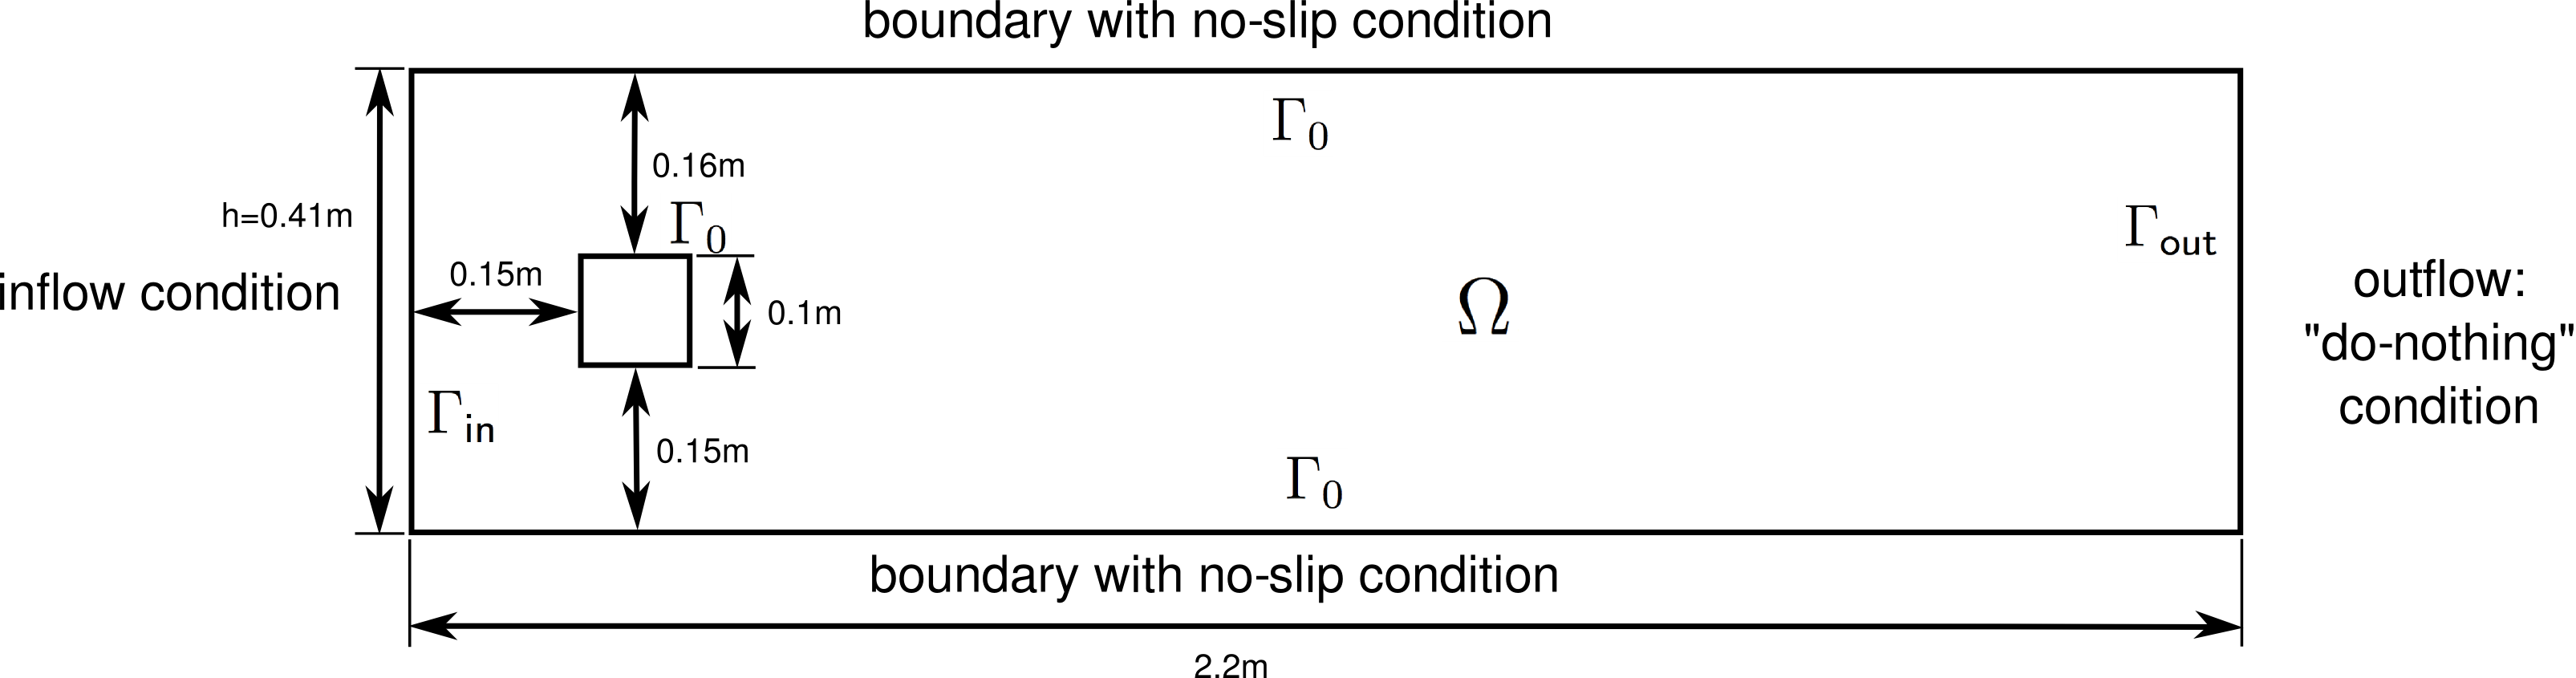
\includegraphics[width=0.9\textwidth]{fig/Zeichnung_Kanal_en.png}
%\caption{Flow channel in 2D.}
%\label{bild1}
%\end{figure}

\section{The Commented Program}

\subsection{Preliminaries}
HiFlow$^3$ is designed for high performance computing on massively parallel machines. 
So it applies the Message Passing Interface (MPI)\index{Message Passing Interface (MPI)}\index{MPI} library specification for message-passing. 
The LES tutorial needs the following two input files:
\begin{itemize}
\item A parameter file: The parameter file is an xml-file, which contains all parameters needed to execute the program. It is read in by the program. Parameters for example defining the termination condition of the non-linear and linear solver are listed as well as parameters needed for the linear algebra. It is not necessary to recompile the program, when parameters in the xml-file are changed. By default the flow tutorial reads in the parameter file les\_tutorial.xml, see section \ref{sectionparameter file}, which contains the parameters of the two-dimensional numerical example, see section \ref{section:numresults}.This file is stored in \verb'/hiflow/examples/les/'. 
\item Geometry data\index{geometry data}: The file containing the geometry is specified in the parameter file. For the numerical results in two dimensions in section \ref{section:numresults} we choose cavity\_les.inp. You can find different meshes in the folder \newline \verb'/hiflow/examples/data' .
\end{itemize}

HiFlow$^3$ does not generate meshes for the domain $\Omega$.\index{domain geometry!generating} Meshes in *.inp and *.vtu format can be read in. There exists a function in \verb'/build/utils/' called 'inp2vtu' which converts *.inp format to *.vtu format. Type \textbf{/build/utils/inp2vtu 2 cavity\_les.inp} to convert cavity\_les.inp to cavity\_les.vtu. Additionally a file cavity\_les\_bdy.vtu is created which shows the body of the domain.\\
It is possible to extend the reader for other formats.
Furthermore it is possible to generate other geometries by using external programs (Mesh generators) or by hand. 
Both formats provide the possibility to mark cell or facets by material numbers.
\subsection{Parameter File}\index{parameter file}\label{sectionparameter file}
The needed parameters are initialized in the parameter file les\_tutorial.xml. The scaling factor $C_S$ is set by the parameter \texttt{TurbulenceParameter}. One can choose the eddy viscosity model from \texttt{Smagorinsky}, \texttt{IliescuLayton1}, \texttt{IliescuLayton2} or \texttt{SUPG} and the LES model between \texttt{Taylor} and \texttt{RationalAux}. Please note that the Taylor LES model is generally unstable and the rational LES model \index{rational!LES model} without an eddy viscosity model also eventually becomes unstable in simulations. $C_S$ should also not be smaller than $\mathcal{O}(0.001)$ to have a meaningful impact of the SGS model. It is possible to leave out the LES model entirely and only specify an eddy viscosity model. 
\begin{lstlisting}[language=XML, basicstyle={\footnotesize, \ttfamily}, keywordstyle=\color{blue}, numbers=none, tabsize=2]
<Param>
    <OutputPrefix>LESTutorial</OutputPrefix>
    <OutputPath>""</OutputPath>
    <Mesh>
        <Filename>cavity_les.inp</Filename>
        <InitialRefLevel>2</InitialRefLevel>
    </Mesh>
    <UseBoundaryDomainDescriptor>0</UseBoundaryDomainDescriptor>
    <FlowModel>
        <Density>1.0</Density>
        <Viscosity>1.e-4</Viscosity>
        <InflowSpeed>1.0</InflowSpeed>
        <InflowHeight>0.41</InflowHeight>
        <InflowWidth>0.41</InflowWidth>
    </FlowModel>
    <DFGbenchmark>0</DFGbenchmark>
    <BenchQuantities>0</BenchQuantities>
    <QuadratureOrder>6</QuadratureOrder>
    <FiniteElements>
        <VelocityDegree>2</VelocityDegree>
        <PressureDegree>1</PressureDegree>
    </FiniteElements>
    <Instationary>
        <SolveInstationary>1</SolveInstationary>
        <Method>CrankNicolson</Method>
        <Timestep>0.005</Timestep>
        <Endtime>20.0</Endtime>
        <TurbulenceParameter>0.005</TurbulenceParameter>
        <EddyViscosityModel>DynamicSmagorinsky</EddyViscosityModel>
        <LESModel>None</LESModel>
    </Instationary>
    <Boundary>
        <InflowMaterial>15</InflowMaterial>
        <OutflowMaterial>16</OutflowMaterial>
        <CylinderMaterial>14</CylinderMaterial>
    </Boundary>
    <NonlinearSolver>
        <UseHiFlowNewton>1</UseHiFlowNewton>
        <MaximumIterations>20</MaximumIterations>
        <AbsoluteTolerance>1.e-15</AbsoluteTolerance>
        <RelativeTolerance>1.e-6</RelativeTolerance>
        <DivergenceLimit>1.e6</DivergenceLimit>
        <ArmijoUpdate>0</ArmijoUpdate>
        <ThetaInitial>1.0</ThetaInitial>
        <ThetaMinimal>1.e-16</ThetaMinimal>
        <ArmijoDecrease>0.5</ArmijoDecrease>
        <SufficientDecrease>1.e-2</SufficientDecrease>
        <MaxArmijoIteration>5</MaxArmijoIteration>
        <ForcingStrategy>EisenstatWalker1</ForcingStrategy>
        <ConstantForcingTerm>1.e-4</ConstantForcingTerm>
        <InitialValueForcingTerm>1.e-3</InitialValueForcingTerm>
        <MaxValueForcingTerm>1.e-2</MaxValueForcingTerm>
        <GammaParameterEW2>0.9</GammaParameterEW2>
        <AlphaParameterEW2>2</AlphaParameterEW2>
    </NonlinearSolver>
    <LinearSolver>
        <MaximumIterations>1000</MaximumIterations>
        <AbsoluteTolerance>1.e-15</AbsoluteTolerance>
        <RelativeTolerance>1.e-6</RelativeTolerance>
        <DivergenceLimit>1.e6</DivergenceLimit>
        <BasisSize>500</BasisSize>
        <Preconditioning>1</Preconditioning>
    </LinearSolver>
    <Schur>
        <NumIter>50</NumIter>
        <RelativeTolerance>1.e-1</RelativeTolerance>
        <PrintLevel>0</PrintLevel>
        <SolverBlockA>
            <NumIter>1000</NumIter>
            <BasisSize>100</BasisSize>
            <RelativeTolerance>5.e-3</RelativeTolerance>
        </SolverBlockA>
        <PrecondBlockA>
            <MaxLevels>25</MaxLevels>
            <MaxCoarseSize>9</MaxCoarseSize>
            <CycleType>1</CycleType>
            <InterpType>6</InterpType>
            <CoarsenType>10</CoarsenType>
            <RelaxType>3</RelaxType>
            <RelaxWt>0.5</RelaxWt>
            <StrongThreshold>0.6</StrongThreshold>
            <NumSweeps>5</NumSweeps>
            <AggNumLevels>25</AggNumLevels>
            <AggInterpType>4</AggInterpType>
            <Nodal>0</Nodal>
            <SmoothNumLevels>0</SmoothNumLevels>
            <Variant>3</Variant>
            <Overlap>1</Overlap>
            <DomainType>1</DomainType>
            <SchwarzUseNonSymm>1</SchwarzUseNonSymm>
        </PrecondBlockA>
        <SolverPrecond>
            <NumIter>500</NumIter>
            <RelativeTolerance>1.e-1</RelativeTolerance>
        </SolverPrecond>
        <PrecondPrecond>
            <MaxLevels>25</MaxLevels>
            <MaxCoarseSize>9</MaxCoarseSize>
            <CycleType>1</CycleType>
            <RelaxType>6</RelaxType>
            <RelaxWt>0.5</RelaxWt>
            <NumFunctions>1</NumFunctions>
            <InterpType>6</InterpType>
            <CoarsenType>10</CoarsenType>
            <StrongThreshold>0.6</StrongThreshold>
            <NumSweeps>3</NumSweeps>
            <AggNumLevels>25</AggNumLevels>
            <AggInterpType>4</AggInterpType>
            <SmoothNumLevels>0</SmoothNumLevels>
            <Variant>3</Variant>
            <Overlap>1</Overlap>
        </PrecondPrecond>
    </Schur>
    <UsePressureFilter>0</UsePressureFilter>
    <Backup>
        <Restore>0</Restore>
        <LastTimeStep>0</LastTimeStep>
        <Filename>backup.h5</Filename>
    </Backup>
</Param>
\end{lstlisting}

\subsection{Member functions}\label{main}\index{MPI}
The main function starts the simulation of the LES problem (les\_tutorial.cc). Most other functions are taken from the HiFlow$^3$ Navier-Stokes tutorial; they will not be discussed here. The boundary conditions are defined in the class ChannelFlowBC (les\_tutorial.h). Note that since the LES auxiliary problems have homogeneous Neumann boundary conditions, these do not have to be explicitly imposed on the weak solution.

\subsubsection{solve()/solve\_eddy\_viscosity\_auxiliary()/solve\_rational\_les\_auxiliary()}\index{solver!non-linear}

The member functions solve(), solve\_eddy\_viscosity\_auxiliary() and solve\_rational\_les\_auxiliary() read in some parameters and solve the non-linear flow problem and the LES auxiliary problems at the current time step. These are implemented in les\_tutorial.cc. The instationary matrix is of course only assembled after setting the parameter $C_S$ of the SGS model and potentially including the solutions of the auxiliary problems. For the first Iliescu-Layton SGS model (\ref{eq:iliLayton}), we filter each velocity component separately and thus define our local assembly (for one version of the model) as follows:   

\begin{lstlisting}[language=C++, basicstyle={\footnotesize, \ttfamily}, keywordstyle=\color{blue},  numbers=none, tabsize=2]
class IliescuLayton1Assembler : private AssemblyAssistant< DIMENSION, double > {
public:
  IliescuLayton1Assembler(const CVector &time_sol) : prev_time_sol_(time_sol) {}

  void set_index(const int var) {
    var_ = var;
  }

  void operator()(const Element< double > &element,
                  const Quadrature< double > &quadrature, LocalMatrix &lm) {
    AssemblyAssistant< DIMENSION, double >::initialize_for_element(element,
        quadrature);

    compute_delta(element);
    // compute local matrix
    const int num_q = num_quadrature_points();
    for(int q = 0; q < num_q; ++q) {
      const double wq = w(q);
      const double dJ = std::abs(detJ(q));
      for(int i = 0; i < num_dofs(0); ++i) {
        for(int j = 0; j < num_dofs(0); ++j) {
          lm(dof_index(i, 0), dof_index(j, 0)) +=
            wq * dot((0.25*delta_*delta_/6.)*grad_phi(j, q), grad_phi(i, q)) * dJ;
        }
      }

      for(int var = 0; var < DIMENSION+1; ++var) {
        const int n_dofs = num_dofs(var);
        for(int i = 0; i < n_dofs; ++i) {
          for(int j = 0; j < n_dofs; ++j) {
            lm(dof_index(i, var), dof_index(j, var)) +=
              wq * phi(j, q, var) * phi(i, q, var) * dJ;
          }
        }
      }
    } // end loop q
  }

  void operator()(const Element< double > &element,
                  const Quadrature< double > &quadrature, LocalVector &lv) {
    AssemblyAssistant< DIMENSION, double >::initialize_for_element(element,
        quadrature);
    // recompute previous timestep velocity for rhs
    for(int d = 0; d < DIMENSION; ++d) {
      vel_ts_[d].clear();
      evaluate_fe_function(prev_time_sol_, d, vel_ts_[d]);
    }

    const int num_q = num_quadrature_points();
    for(int q = 0; q < num_q; ++q) {
      const double wq = w(q);
      const double dJ = std::abs(detJ(q));

      for(int i = 0; i < num_dofs(0); ++i) {
        lv[dof_index(i, 0)] += wq * vel_ts_[var_][q] * phi(i, q) * dJ;
      }
    }
  }
private:

  void compute_delta(const Element< double > &element) {
    const mesh::Entity cell = element.get_cell();
    const mesh::TDim edge_dim = 1;

    delta_ = h();
    std::vector<double> edge_coords;
    for(mesh::IncidentEntityIterator it = cell.begin_incident(edge_dim);
        it != cell.end_incident(edge_dim); ++it) {
      it->get_coordinates(edge_coords);
      delta_ = std::min(delta_,sqrt(std::pow(edge_coords[0]-edge_coords[2],
                                             2)+std::pow(edge_coords[1]
                                             -edge_coords[3],2)));
    }
    delta_ *= 2.; // 2 * shortest edge of cell
  }

  int var_; // velocity component for which the scalar Helmholtz equation is solved
  const CVector &prev_time_sol_;
  double delta_;
  FunctionValues < double > vel_ts_[DIMENSION]; // velocity at previous timestep
};
\end{lstlisting}

As the rational LES auxiliary problem is actually tensor-valued, we would in theory have to solve $d^2$ scalar Helmholtz problems. Fortunately, the tensor $\nabla w \nabla w^T$ is symmetric. Therefore, only $\frac{d(d+1)}{2}$ auxiliary equations have to be solved. The class of the local assembler for the rational LES term is then

\begin{lstlisting}[language=C++, basicstyle={\footnotesize, \ttfamily}, keywordstyle=\color{blue},  numbers=none, tabsize=2]
class RationalLESAssembler : private AssemblyAssistant< DIMENSION, double > {
public:
  RationalLESAssembler(const CVector &time_sol) : prev_time_sol_(time_sol) {}

  void set_indices(int var_i, int var_j) {
    var_i_ = var_i;
    var_j_ = var_j;
  }

  void operator()(const Element< double > &element,
                  const Quadrature< double > &quadrature, LocalMatrix &lm) {
    AssemblyAssistant< DIMENSION, double >::initialize_for_element(element,
        quadrature);

    compute_delta(element);
    // compute local matrix
    const int num_q = num_quadrature_points();
    for(int q = 0; q < num_q; ++q) {
      const double wq = w(q);
      const double dJ = std::abs(detJ(q));
      for(int i = 0; i < num_dofs(0); ++i) {
        for(int j = 0; j < num_dofs(0); ++j) {
          lm(dof_index(i, 0), dof_index(j, 0)) +=
            wq * dot((0.25*delta_*delta_/6.)*grad_phi(j, q), grad_phi(i, q)) * dJ;
        }
      }

      for(int var = 0; var < DIMENSION+1; ++var) {
        const int n_dofs = num_dofs(var);
        for(int i = 0; i < n_dofs; ++i) {
          for(int j = 0; j < n_dofs; ++j) {
            lm(dof_index(i, var), dof_index(j, var)) +=
              wq * phi(j, q, var) * phi(i, q, var) * dJ;
          }
        }
      }
    } // end loop q
  }
  
  void operator()(const Element< double > &element,
                  const Quadrature< double > &quadrature, LocalVector &lv) {
    AssemblyAssistant< DIMENSION, double >::initialize_for_element(element,
        quadrature);
    // recompute previous timestep velocity for rhs
    for(int d = 0; d < DIMENSION; ++d) {
      grad_vel_ts_[d].clear();
      evaluate_fe_function_gradients(prev_time_sol_, d, grad_vel_ts_[d]);
    }

    compute_delta(element);
    const int num_q = num_quadrature_points();

    for(int q = 0; q < num_q; ++q) {
      const double wq = w(q);
      const double dJ = std::abs(detJ(q));
      // Get previous timestep velocity gradient times its transpose
      for(int i = 0; i < num_dofs(0); ++i) {
        lv[dof_index(i, 0)] += wq * (0.5*delta_*delta_/6.) * dot(
                                 grad_vel_ts_[var_i_][q],grad_vel_ts_[var_j_][q])
                                 * phi(i, q) * dJ;
      }
    }
  }
private:

  void compute_delta(const Element< double > &element) {
    const mesh::Entity cell = element.get_cell();
    const mesh::TDim edge_dim = 1;

    delta_ = h();
    std::vector<double> edge_coords;
    for(mesh::IncidentEntityIterator it = cell.begin_incident(edge_dim);
        it != cell.end_incident(edge_dim); ++it) {
      it->get_coordinates(edge_coords);
      delta_ = std::min(delta_,sqrt(std::pow(edge_coords[0]-edge_coords[2],
                                             2)+std::pow(edge_coords[1]
                                             -edge_coords[3],2)));
    }
    delta_ *= 2.; // 2 * shortest edge of cell
  }

  int var_i_;
  int var_j_; // component of velocity gradient times transpose 
              // for which the scalar Helmholtz equation is solved
  const CVector &prev_time_sol_;
  double delta_;
  FunctionValues < Vec < DIMENSION, double > >
  grad_vel_ts_[DIMENSION]; // gradient of velocity at previous timestep

};

\end{lstlisting}

\section{Program Output}
HiFlow$^3$ can be executed in a parallel or sequential mode which influence the generated output data. Note that the log files can be viewed by any editor.
\subsection{Parallel Mode}\index{parallel mode}
Executing the program in parallel, for example with four processes by \textbf{mpirun -np 4 ./les\_tutorial}  \index{program!executing in parallel} 
generates following output data. 

\begin{itemize}
\item Mesh/geometry data:
\begin{itemize}
\item \textbf{mesh\_local.pvtu} Global mesh (parallel vtk-format). It combines the local meshes of sequential vtk-format owned by the different processes to the global mesh.
\item \textbf{mesh\_local\_X.vtu} local mesh owned by process X for X=0, 1, 2 and 3 (vtk-format).
\end{itemize}

\item Solution data. Since it is only possible to visualize data of polynomial degree 1 ($Q_1$ on quads in 2 dimensions), 
only the data corresponding to the degrees of freedom of a $Q_1$ element are written out. 
It means the information of the degrees of freedom of higher order is lost due to the fact that it cannot be visualized using the vtk-format.

\begin{itemize}
\item \textbf{LESTutorial\_solution\_.pvtu} Solution of the velocity field and the pressure variable (parallel vtk-format). It combines the local solutions owned by the different processes to a global solution.
\item \textbf{LESTutorial\_solution\_X.vtu} Local solution of the velocity field and the pressure variable of the degrees of freedoms which belong to cells owned by process X, for X=0, 1, 2 and 3 (vtk-format).
\end{itemize}
\item Log files:
\begin{itemize}
\item \textbf{LESTutorial\_debug\_log} Log file listing errors helping to simplify the debugging process. This file is empty if the program runs without errors.
\item \textbf{LESTutorial\_info\_log} Log file listing parameters and some helpful informations to control 
      the program as for example information about the residual of the linear and non-linear solver used.
\end{itemize}
\end{itemize}

\subsection{Sequential Mode}\index{sequential mode}
Executing the program sequentially by \textbf{./les\_tutorial} following output data is generated.\index{program!executing sequentially} 
\begin{itemize}
\item Mesh/geometry data:
\begin{itemize}
\item \textbf{mesh\_local.pvtu} Global mesh (parallel vtk-format). 
\item \textbf{mesh\_local\_0.vtu} Global mesh owned by process 0 (vtk-format) containing the mesh information.
\end{itemize}
\item Solution data. Since it is only possible to visualize data of polynomial degree 1 (Q1 on quads in 2 dimensions), only the data corresponding to the degrees of freedom of a Q1-element are written out. It means the information of the degrees of freedom of higher order are lost due to the fact that this information cannot be visualized using the vtk-format.
\begin{itemize}
\item \textbf{LESTutorial\_solution.vtu} Solution of the velocity field and the pressure variable (vtk-format). 
\end{itemize}
\item Log files:
\begin{itemize}
\item \textbf{LESTutorial\_debug\_log} is a list of errors helping to simplify the debugging process. This file keeps empty if the program runs without errors.
\item \textbf{LESTutorial\_info\_log} is a list of parameters and some helpful informations to control the program as for example information about the residual of the linear and non-linear solver used.
\end{itemize}
\end{itemize}

\subsection{Visualizing the Solution}\index{visualization}
HiFlow$^3$ only generates output data but does not visualize. The mesh/geometry data as well as the solution data can be visualized 
by any external program which can handle the vtk data format as e.g. the program ParaView \cite{Paraview}.\index{paraview} 

\section{Numerical Example}

\subsection{Driven cavity}\label{section:numresults}

\begin{figure}[!ht]
	\centering
	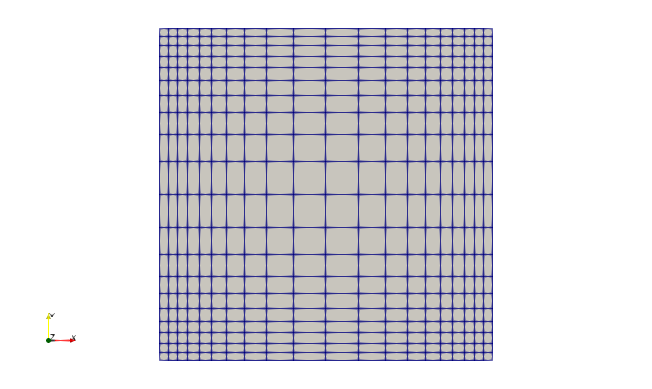
\includegraphics[scale=0.5]{./fig/les_mesh.png}
	\caption{The mesh (cavity\_les.inp) used for the simulation is finer toward the walls. For our example simulation, it is refined twice.}
	\label{mesh_cavity}
\end{figure}

We set $U_m = 1.0 ms^{-1}$ and $H=1.0m$ in the parameter file. As geometry data we choose the square mesh with refinement towards the walls given by cavity\_les.inp. The inflow condition $g(x,1)$ at the top (inflow boundary $\Gamma_{\text{in}}$) is a regularized version of the well-known lid-driven cavity problem (see \cite{DEFRUTOS2016368} for details) and defined as

\begin{equation}
g(x,1) = \begin{pmatrix}
         g_1(x) \\ 0
         \end{pmatrix},
\end{equation}

\begin{equation}
 g_1(x) = \begin{cases}
          1 - \frac{1}{4}\big(1-\mathrm{cos}\big(\frac{x_1-x}{x_1}\pi\big)\big)^2 & \mathrm{for } x \in [0,x_1], \\
          1 & \mathrm{for } x \in (x_1, 1-x_1), \\
          1-\frac{1}{4}\big(1-\mathrm{cos}\big(\frac{1-(1-x_1)}{x_1}\pi\big)\big)^2 & \mathrm{for } x \in [1-x_1,1]
          \end{cases}
\end{equation} 

with $x_1 = 0.1$. All other walls have no-slip / homogeneous Dirichlet boundary conditions. Because these boundary conditions are not implemented by material numbers, you do not have to change the material numbers in the parameter file. As one example, fig. \ref{mesh_cavity}-\ref{pressure_cavity} show the mesh, the solution on refinement level 2 for this example illustrated by the magnitude of the velocity vector and the
pressure for the parameters $\text{Re} = 10^5$ and $C_S = 0.1$ with the first Iliescu-Layton model.  

\begin{figure}[!ht]
	\centering
	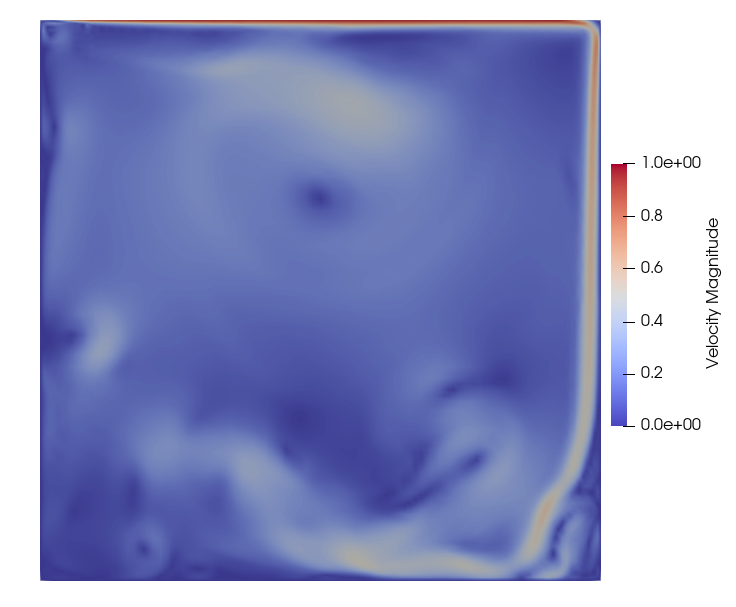
\includegraphics[scale=0.35]{./fig/vili.png}
\caption{The magnitude of the velocity vector field $w_h \in U_h(\Omega)$ of the simulation.}
\label{sol_cavity}
\end{figure}

\begin{figure}[!ht]
	\centering
	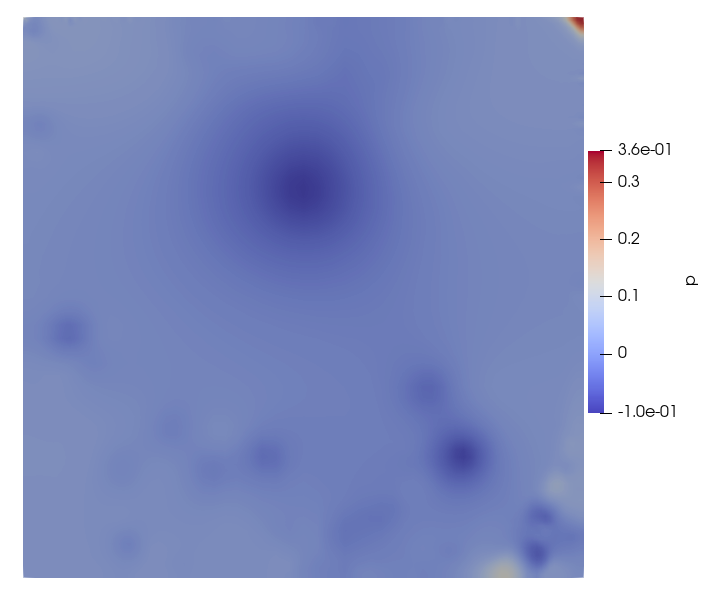
\includegraphics[scale = 0.35]{./fig/pili.png}
\caption{The solution for the pressure.}
\label{pressure_cavity}
\end{figure}

\newpage
\appendix
\bibliography{tutorials_bib}
\bibliographystyle{plain}

\printindex

\end{document}
